% \chapter{Statistics}\label{chap:statistics}
% \section{Random Variables and Probability Distributions}\label{sec:pdfs}
% Random variables can describe either discrete variables, such as the result from throwing a dice, or continuous variables such as measuring a distance. In order to learn about the likelihood that a random variable has a certain outcome, we can repeat the experiment many times and record the resulting \emph{random variates}\index{Variate (Random variable)}, that is the actual values of the random variable, and the number of times they occurred. For a perfectly cubic dice we will see that the random variable can hold natural numbers from 1 to 6, that have the same likelihood of 1/6.

% The function that describes the probability of a random variable to take certain values is called a \emph{probability distribution}\index{Probability Distribution}.
% As the likelihood of all possible random variates in the dice experiment is the same, the dice follows what we call a \emph{uniform distribution}\index{Uniform Distribution}. More accurately, as the outcomes of rolling a dice are discrete numbers, it is actually a discrete uniform distribution. Most random variables are not uniformly distributed, but some variates are more likely than others. For example, when considering a random variable that describes the sum of two simultaneously thrown dice, we can see that the distribution is anything but uniform:

\chapter{统计}
\label{chap:statistics}
\section {随机变量和概率分布} 
\label{sec:pdfs}
随机变量可以描述离散变量,例如投掷骰子的结果,或连续变量,如测量距离。为了了解随机变量有一定的结果的可能性,我们可以多次重复实验,并记录生成的\emph{随机变量(Random variates)}\index{Variate(Random variable)},即实际值随机变量及其发生次数。对于一个完美的立方体骰子,我们将看到随机变量可以保持1到6的自然数,这与1/6相同。

描述随机变量采取某些值的概率的函数称为\emph{概率分布(Probability distribution)}\index{概率分布(Probability distribution)}。
由于骰子实验中所有可能的随机变量的可能性是相同的,所以骰子跟随我们所说的\emph{均匀分布(Uniform Distribution)}\index{均匀分布(Uniform Distribution)}。更准确地说,由于骰子滚动的结果是离散数字,实际上是一个离散的均匀分布。大多数随机变量不均匀分布,但有些变量比其他变量更有可能。例如,当考虑描述两个同时投掷的骰子的总和的随机变量时,我们可以看到分布是均匀的:

$\begin{array}{ll}
2: 1+1 & \rightarrow \frac{1}{6}\frac{1}{6}\\
3: 1+2, 2+1 &\rightarrow 2\frac{1}{6}\frac{1}{6}\\
4: 1+3, 2+2, 3+1 &\rightarrow 3\frac{1}{6}\frac{1}{6}\\
5: 1+4, 2+3, 3+2, 4+1 & \rightarrow 4\frac{1}{6}\frac{1}{6}\\
6: 1+5, 2+4, 3+3, 4+2, 5+1 & \rightarrow 5\frac{1}{6}\frac{1}{6}\\
7: 1+6, 2+5, 3+4, 4+3, 5+2, 6+1 & \rightarrow 6\frac{1}{6}\frac{1}{6}\\
8: 2+6, 3+5, 4+4, 5+3, 6+2 & \rightarrow 5\frac{1}{6}\frac{1}{6}\\
9: 3+6, 4+5, 5+4, 6+3 & \rightarrow 4\frac{1}{6}\frac{1}{6}\\
10: 4+6, 5+5, 6+4 & \rightarrow 3\frac{1}{6}\frac{1}{6}\\
11: 5+6, 6+5 & \rightarrow 2\frac{1}{6}\frac{1}{6}\\
12: 6+6 & \rightarrow \frac{1}{6}\frac{1}{6}\\
\end{array}$

% As one can see, there are many more possibilities to sum up to a 7 than there are to a 3, e.g. While it is possible to store probability distributions such as this one as a look-up table to predict the outcome of an experiment (or that of a measurement), we can also calculate the sum of two random processes analytically (Section \ref{sec:convolution}). 

可以看出,有更多的可能性总结到7比3,例如。虽然可以存储像这样的概率分布作为查找表来预测实验的结果(或测量的结果),但是我们也可以分析地计算两个随机过程的和(Section\ref{sec:convolution})。

% \subsection{The Normal Distribution}
% One of the most prominent distribution is the Gaussian or Normal Distribution. The \emph{Normal distribution}\index{Normal Distribution}\index{Gaussian Distribution} is characterized by a \emph{mean} and a \emph{variance}. Here, the mean corresponds to the average value of a random variable (or the peak of the distribution) and the variance is a measure of how broadly variates are spread around the mean (or the width of the distribution).

% The Normal distribution is defined by the following function

\subsection{正态分布}
最突出的分布之一是高斯分布或正态分布。\emph{正态分布(Normal distribution)}\index{正态分布(Normal Distribution)}\index{高斯分布(Gaussian Distribution)}的特征在于\emph{均值(mean)}和\emph{方差(variance)}。 这里,平均值对应于随机变量(或分布的峰值)的平均值,方差是变量在平均值(或分布宽度)周围扩散的度量。

正态分布由以下功能定义

\begin{equation}
f(x)=\frac{1}{\sqrt{2\pi\sigma^2}}e^{-\frac{(x-\mu)^2}{2\sigma^2}}
\end{equation}

% where $ \mu$ is the mean and $ \sigma^2$ the variance. ($ \sigma$ on its own is known as the standard deviation.) Then, $ f(x)$ is the probability for a random variable $ X$ to have value $ x$.

其中$\mu$是平均值,$\sigma^2$的方差。($\sigma$自己被称为标准偏差。)然后,$f(x)$是随机变量$X$的值为$x$的概率。

\begin{figure}
	\centering
		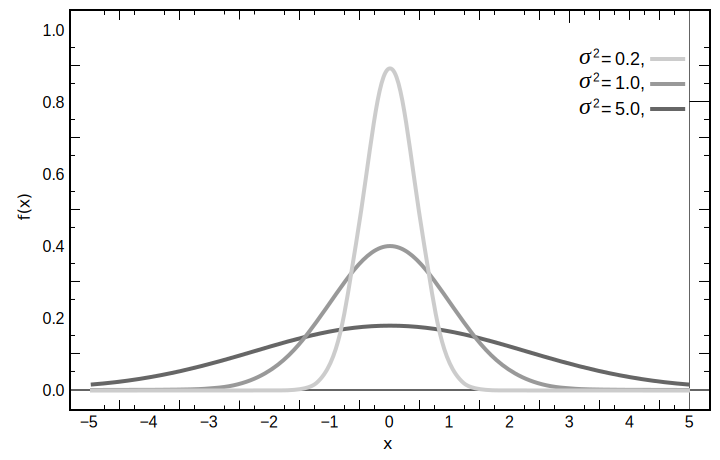
\includegraphics[width=\textwidth]{figs/Normal_Distribution_PDF}
	% \caption{Normal distribution for different variances and $\mu=0$.}
	\caption{不同方差的正态分布,$\mu=0$。}
	\label{fig:Normal_Distribution_PDF}
\end{figure}

% The mean is calculated by

平均值由...计算

\begin{equation}
\mu=\int_{-\infty}^{\infty}xf(x)dx
\end{equation}

% or in other words, each possible value $ x$ is weighted by its likelihood and added up.

% The variance is calculated by

或者换句话说,每个可能的值$x$由其可能性加权并加起来。

方差计算

\begin{equation}
\sigma^2=\int_{-\infty}^{\infty}(x-\mu)^2f(x)dx
\end{equation}

% or in other words, we calculate the deviation of each random variable from the mean, square it, and weigh it by its likelihood. Although it is tantalizing to perform this calculation also for the double dice experiment, the resulting value is questionable, as the double dice experiment does not follow a Normal distribution. We know this, because we actually enumerated all possible outcomes. For other experiments, such as grades in the classes you are taking, we don't know what the real distribution is.

或者换句话说,我们计算每个随机变量与平均值的平方,它的平方和它的可能性。尽管对于双重骰子实验也可以进行这种计算,但是由于双骰子实验不遵循正态分布,所以得到的值是值得怀疑的。我们知道这一点,因为我们实际上列举了所有可能的结果。对于其他实验,例如您正在学习的课程中的成绩,我们不知道真正的分配是什么。

% \subsection{Normal distribution in two dimensions}
% The Normal Distribution is not limited to random processes with only one random variable. For example, the X/Y position of a robot in the plane is a random process with two dimensions. In case of a multi-variate distribution with $k$ dimensions, the random variable $ X$ is a k-dimensional vector of random variables, $ \mu$ is a k-dimensional vector of means, and $ \sigma$ gets replaced with $ \Sigma$,  a k-by-k dimensional \emph{covariance matrix}\index{Covariance Matrix} (a matrix that carries the variances of each random variable in its diagonal).

\subsection{二维正态分布}
正态分布不限于只有一个随机变量的随机过程。例如,机器人在平面中的$X/Y$位置是具有二维的随机过程。在具有$k$维度的多变量分布的情况下,随机变量$X$是随机变量的k维向量,$\mu$是平均值的$k$维向量,$\sigma$被替换与$\Sigma$,一个$k-k$维\emph{协方差矩阵(Covariance Matrix)}\index{协方差矩阵(Covariance Matrix)}(一个矩阵,其携带每个随机变量在其对角线中的方差)。

% \section{Conditional Probabilities and Bayes Rule}\label{sec:bayesrule}
% Let $A$ and $B$ be random events with probabilities $P(A)$ and $P(B)$. We can now say that the probability $P(A \cap B)$ that event $A$ \emph{and} $B$ happen is given by

\section{条件概率和贝叶斯规则}
\label{sec:bayesrule}
令$A$和$B$是概率为$P(A)$和$P(B)$的随机事件。我们现在可以说,事件$A$\emph{和}$B$发生的概率$P(A\cap B)$是由

\begin{equation}\label{eq:conditionalprob}
P(A \cap B)=P(A)P(B|A)=P(B)P(A|B)
\end{equation}

% Here, $P(B|A)$ is the \emph{conditional probability}\index{Conditional Probability} that $B$ happens, knowing that event $A$ happens. Likewise, $P(A|B)$ is the probability that event $A$ happens given that $B$ happens.

% Bayes' Rule\index{Bayes' Rule} relates a conditional probability to its inverse. In other words, if we know the probability of event $A$ to happen given that event $B$ is happening, we can calculate the probability of $B$ to occur given that $A$ is happening. Bayes' rule can be derived from the simple observation that the probability of $A$ and $B$ to happen together ($P(A \cap B)$) is given by $P(A)P(B|A)$ or the probability of $A$ to happen and the probability of $B$ to happen given that $A$ happens (Equation \ref{eq:conditionalprob}). 
% From this, deriving Bayes' rule is straightforward:

在这里,$P(B|A)$是知道$A$事件的$B$发生的\emph{条件概率(Conditional Probability)}\index{条件概率(Conditional Probability)}。同样,$P(A|B)$是$B$发生的事件$A$的概率。

贝叶斯规则\index{贝叶斯规则(Bayes' Rule)}将条件概率与其逆向相关联。换句话说,如果我们知道事件$A$发生事件$B$发生的概率,我们可以计算$A$发生的概率,因为$A$正在发生。贝叶斯规则可以从简单的观察得出,$A$和$B$发生在一起的概率($P(A\cap B)$)由$P(A)P(B|A)$或者$A$发生的概率以及$A$发生的概率(等式\ref{eq:conditionalprob}))。

从此,得出贝叶斯的规则是直截了当的:

\begin{equation}
P(A|B)=\frac{P(A)P(B|A)}{P(B)}
\end{equation}

% In words, if we know the probability that $B$ happens given that $A$ happens, we can calculate that $A$ happens given that $B$ happens. 

换句话说,如果我们知道$A$发生的概率是$A$发生,我们可以计算出$A$发生在$B$发生时发生。

% \section{Sum of two random processes}\label{sec:convolution}
% Let $X$ and $Y$ be the random variables associated with the numbers shown on two dice (see above), and $Z=X+Y$. With $P(X=x)$, $P(Y=y)$, and $P(Z=z)$ being the probabilities associated with the random variables taking specific values $x,y$ or $z$. Given $z=x+y$, the event $Z=z$ is the union of the independent events $X=k$ and $Y=z-k$. We can therefore write

\section{两个随机过程的总和}
\label{sec:convolution}
让$X$和$Y$是与两个骰子(见上文)上显示的数字相关联的随机变量,$Z=X+Y$。使用$P(X=x)$,$P(Y=y)$和$P(Z=z)$是与使用特定值$x,y$或$z$的随机变量相关联的概率。给定$z=x+y$,事件$Z=z$是独立事件$X=k$和$Y=z-k$的并集。所以我们可以写

\begin{equation}
P(Z=z)=\sum_{k=-\infty}^{\infty}P(X=k)P(Y=z-k)
\end{equation}

% which is the exact definition of a \emph{convolution}\index{Convolution}, also written as 

这是\emph{卷积(Convolution)}\index{卷积(Convolution)}的确切定义,也写为

\begin{equation}
P(Z)=P(X)\star P(Y)
\end{equation}

% Numerically calculating the convolution always works, and can be done analytically for some probability distributions. 

% Conveniently, the convolution of two Gaussian distributions is again a Gaussian distribution with a variance that corresponds to the sum of the variances of the indivdiual Gaussians. 

数值计算卷积总是有效的,并且可以通过分析来完成某些概率分布。

方便地,两个高斯分布的卷积又是一个高斯分布,其方差对应于不同高斯的方差之和。

% \section{Linear Combinations of Independent Gaussian Random Variables}\label{sec:lcombrandom}
% Let $X_1$, $X_2$, $\ldots$, $X_n$ be $n$ independent random variables with means $\mu_1$, $\mu_2$, $\ldots$, $\mu_n$ and variances $\sigma_1^2$, $\sigma_2^2$, $\ldots$, and $\sigma^2_n$. Let $Y$ be a random variable that is a linear combination of $X_i$ with weights $a_i$ so that $Y=\sum_{i=1}^na_iX_i$. 

% As the sum of two Gaussian random variables is again a Gaussian, $Y$ is Gaussian distributed with a mean 

\section{独立高斯随机变量的线性组合}\label{sec:lcombrandom}
让$X_1$,$X_2$,$\ldots$,$X_n$为$n$独立的随机变量,意思是$\mu_1$,$\mu_2$,$\ldots$,$\mu_n$和差异$\sigma_1^2$,$\sigma_2^2$,$\ldots$和$\sigma^2_n$。让$Y$是一个随机变量,它是$X_i$与权重$a_i$的线性组合,以便$Y=\sum_{i=1}^na_iX_i$。

由于两个高斯随机变量的和又是一个高斯,所以$Y$是高斯分布的平均值

\begin{equation}
\mu_Y=\sum_{i=1}^na_i\mu_i
\end{equation}
and a variance
\begin{equation}
\sigma_Y^2=\sum_{i=1}^na_i^2\sigma_i^2
\end{equation}  


% \section{Testing Statistical Significance}
% \label{sec:stattest}
% Robotics is an experimental discipline. This means that algorithms and systems you develop need to be validated by real hardware experiments. Doing an experiment to validate your hypothesis is at the core of the scientific method and doing it right is a discipline on its own. The key is to show that your results is not simply a result of chance. In practice, this is impossible to show. Instead, it is possible to express the likelihood that your results have not been obtained by chance. This is known as the statistical significance level. How to calculate the statistical significance level depends on the problem you are studying. This section will introduce three common problems in robotics:

\section{检验统计意义}
\label{sec:stattest}
机器人是一个实验纪律。这意味着您开发的算法和系统需要通过实际的硬件实验验证。做一个验证你的假设的实验是科学方法的核心,正确的是一个学科自己。关键是要表明你的结果不仅仅是机会的结果。在实践中,这是不可能显示的。相反,可以表示您的结果并不是偶然获得的可能性。这被称为统计显着性水平。如何计算统计显着性水平取决于您正在研究的问题。本节将介绍机器人技术中的三个常见问题:

\begin{enumerate}
% \item testing whether data is indeed distributed according to a specific distribution
% \item testing whether two sets of data are generated from different distributions
% \item testing whether true-false experiments are a sequence of luck or not

\item 测试数据是否确实根据具体的分布进行分发
\item 测试是否从不同的分布生成两组数据
\item 测试是否真假实验是一系列运气与否
\end{enumerate}

% \subsection{Null Hypothesis on Distributions}
% The Null Hypothesis is a term from the statistical significance literature and formally captures your main claim. A statistical test can either reject the Null Hypothesis or fail to reject it. It can never be proven as there will always be a non-zero probability that all your experiments are just a lucky coincidence. The statistical significance level of a Null Hypothesis is known as the p-value.

% An import class of Null Hypothesis are on the distribution of data. Consider the following example from Lab 1 (message passing in ROS). Students were asked to experimentally study the time it takes to pass a message from one process to another:

\subsection{分布上的空假设}
空假设是统计学意义文献中的一个术语,并正式捕获了您的主要要求。统计测试可以拒绝Null假设,也可以拒绝它。它永远不会被证明,因为总是有一个非零概率,所有的实验只是一个幸运的巧合。空假设的统计显着性水平被称为p值。

零假设的进口类别是数据分布。请考虑实验1中的以下示例(ROS中的消息传递)。要求学生实验研究将消息从一个过程传递给另一个过程所需的时间:

\begin{framed}
% Histogram of the time it takes to send a ROS message from one process to another based on 10 trials.

基于10次试验,将ROS消息从一个进程发送到另一个进程的时间的直方图。
\end{framed}

% We observe three peaks in this Histogram. What can we say about message passing times? For example

我们在这个直方图中观察到三个峰。 我们可以说什么消息传递时间? 例如

\begin{itemize}
% \item H0: Message passing times follow a Gaussian distribution.
% \item H0: Message passing times follow a bi-modal distribution.
% \item H0: Message passing times follow a log-normal distribution.

\item H0:消息传递时间遵循高斯分布。
\item H0:消息传递时间遵循双模态分布。
\item H0:消息传递时间遵循对数正态分布。
\end{itemize}

% The first Null Hypothesis implies that messages take sometimes a little longer and sometimes a little shorter, but have an average and a variance. The second Null Hypothesis implies that usually messages take some low average time, but occasionally are delayed due to the influence of some other process, for example operating system duties. You can now test each of these hypotheses by calculating the parameters of the distribution to expect and calculate the joint probability that each of your measurements are actually drawn from this distribution. You will find, that all of the above hypotheses are almost equally likely. Together, none of your tests will reject your hypothesis. You therefore will need more data:

第一个空假设意味着消息有时会更长一些,有时更短一点,但是有一个平均值和方差。第二个Null假设意味着通常消息需要一些较低的平均时间,但是由于某些其他过程的影响,例如操作系统的任务,偶尔会被延迟。您现在可以通过计算预期分布的参数来测试这些假设,并计算每个测量值实际上来自该分布的联合概率。你会发现,所有上述假设几乎同样可能。一起,你的测试都不会拒绝你的假设。因此,您将需要更多数据:

\begin{framed}
% Histogram of message passing times in ROS based on a 1000 trials.

基于1000次试验的ROS中消息传递时间的直方图。
\end{framed}

% You can now again calculate parameters for each distribution you suspect. For example, you can calculate the mean and variance of this data and plot the resulting Gaussian distribution. In this example, the Gaussian distribution will have a mean slightly offset to the right of the peak. You can also fit the data to a log-normal distribution. You can now calculate the likelihood for the data actually be drawn from either of the two distributions. You will see that the joint probability (the product of all likelihoods) for all data points is actually much higher than that for any Gaussian distribution or any bimodal distribution that you are able to fit.

% Formally, this can be done by following Pearsons $ \chi^2$-Test (read Chi-Squared Test). This test calculates a value that will approximate a $ \chi^2$-distribution from all samples and the likelihood of that sample based on the expected distribution. Plugging the resulting value into the $ \chi^2$-distribution leads to the statistical significance level (or p-value).

% The value of the test-statistic is calculated as follows:

您现在可以再次计算您怀疑的每个分发的参数。例如,您可以计算该数据的平均值和方差,并绘制所得到的高斯分布。在这个例子中,高斯分布的平均值稍微偏移到峰的右边。您也可以将数据适合于对数正态分布。您现在可以计算实际从两个分布中的任一个绘制数据的可能性。您将看到所有数据点的联合概率(所有可能性的乘积)实际上远高于您能够适应的任何高斯分布或任何双峰分布。

正式地,这可以通过以下Pearsons$\chi^2$-Test(读卡方检验)来完成。此测试计算将从所有样本近似$\chi^2$-distribution的值,以及基于预期分布的样本的可能性。将结果值插入到$\chi^2$-distribution中会导致统计显着性级别(或p值)。

测试统计量的值计算如下:

\begin{equation}
\chi^2 = \sum_{i=1}^{n} \frac{(O_i - E_i)^2}{E_i}
\end{equation}

% where
其中

\begin{itemize}
% \item $ \chi^2$ = Pearson's cumulative test statistic, which asymptotically approaches a chi-squared distribution.
% \item $ O_i$ = an observed frequency in the data histogram
% \item $ E_i$ = an expected (theoretical) frequency, asserted by the null hypothesis, i.e., the distribution you think the data should follow
% \item n = the number of samples.

\item $\chi^2$=Pearson的累积测试统计量,其渐近地接近卡方分布。
\item $O_i$=数据直方图中观察到的频率
\item $E_i$=一个预期(理论)频率,由零假设声明,即您认为数据应遵循的分布
\item $n$=样本数。
\end{itemize}

% This example also illustrates how statistical tests can be used to determine if you have enough data. If you don't, you will get very poor p-values.  In practice, it is up to you what likelihood you determine to be significant. Standard significance levels are 10\%, 5\% and 1\%. If you are unsatisfied with your p-values you can collect more data and check, whether your p-value improves.

此示例还说明如何使用统计测试来确定是否有足够的数据。如果你不这样做,你会得到很差的p值。在实践中,由你决定是重要的可能性取决于你。标准显着性水平为$10\%$,$5\%$,$1\%$。如果您不满意您的p值,您可以收集更多数据并检查您的p值是否改善。

% \subsection{Testing whether two distributions are independent}
% Testing whether the data of two experiments are independent is probably the most common statistical test. For example, you might run 10 experiments using algorithm 1 and 10 experiments using algorithm 2. It is up to you to show that the resulting distributions are indeed statistically significantly different. In other words, you need to show that the differences between the algorithm indeed lead to a systematic improvement, and that it was not purely luck that one set of experiments turned out ``better'' than another.

% If you have good reasons to believe that your data is normal distributed, there exist a series of simple tests. For example, to test whether two sets of data are distributed with Gaussian distributions that have the same mean, can be done using Student's t-test. A generalization of Student's t-test to 3 or more groups is ANOVA. These tests have to be done with care as most distributions in robotics are not normal distributed. Examples where  Gaussian distributions are commonly assumed are sensor noise on distance measurements such as obtained by infrared or odometry.

% If data is not Gaussian distributed, there exist a series of numerical tests to test the likelihood that two distributions are independent. For example, you could test the message passing time with and without running some computationally expensive image processing routines. You can then test whether the additional computation affects message passing time. If it does, both distributions need to be significantly different. Just using Student's t-test does not work as the distributions are not Gaussian!

% Instead, testing whether two sets of data have the same mean, needs to be done numerically. A common test is Mann-Wilcoxon's Ranked Sum test. An implementation of this test is part of most mathematical calculation programs such as Matlab or Mathematica. An algorithm to calculate this test statistic and the corresponding p-values is available on the Wikipedia page above. An extension of the Mann-Wilcoxon's Ranked Sum test for 3 or more groups is the Kruskal-Wallis one-way analysis of variance test.

\subsection{测试两个分布是否独立}
测试两个实验的数据是否独立可能是最常见的统计测试。例如,您可以使用算法1运行10次实验,并使用算法2进行10次实验。由您来证明所得到的分布在统计上显着不同。换句话说,你需要表明,算法之间的差异确实导致了系统的改进,而不是纯粹的运气,一组实验比另外一种更好。

如果您有足够的理由相信您的数据是正态分布的,则会出现一系列简单的测试。例如,为了测试两组数据是否具有相同均值的高斯分布,可以使用Student t检验来完成。对3人以上学生的t检验的概括是方差分析。这些测试必须小心,因为大多数机器人分析不是正态分布。通常假设高斯分布的实例是距离测量的传感器噪声,例如通过红外或距离测量得到的。

如果数据不是高斯分布,则存在一系列数值测试来测试两个分布是独立的可能性。例如,您可以使用和不运行一些计算上昂贵的图像处理例程来测试消息传递时间。然后,您可以测试附加计算是否影响消息传递时间。如果是这样,两个分发都需要有很大的不同。只要使用学生的t检验不起作用,因为分布不是高斯!

相反,测试两组数据是否具有相同的平均值,需要在数字上进行。一个常见的测试是Mann-Wilcoxon的排名和测试。该测试的实现是大多数数学计算程序的一部分,如Matlab或Mathematica。计算此测试统计量和相应p值的算法可在上面的维基百科页面获得。对于3个或更多个组,Mann-Wilcoxon的Rank-Sum测试的扩展是Kruskal-Wallis单向方差分析测试。


% \subsection{Statistical Significance of True-False Tests}
% There exists a class of experiments that do not lead to distributions, but result in simple true-false outcomes. For example, a question one might ask is ``does the robot correctly understand a spoken command''. This class of experiments is captured by the Lady tasting tea example. Here, a lady claims that she can identify the brewing method of a cup of tea: tea prepared by first adding milk and tea prepared by later adding milk. Unfortunately, it is easy to cheat as the likelihood of guessing right is 50\%. Testing the hypothesis that the lady can indeed differentiate the two brewing methods therefore requires to conduct a series of experiments to reduce the likelihood of winning by guesswork. In order to do this, one needs to calculate the number of total permutations (or, possible outcomes over the entire series of experiments). For example, one could present the lady 8 cups of tea, 4 brewed one way and four the other. One can now enumerate all possible outcomes of this experiment, ranging from all cups guessed correctly to all cups guessed wrong. There are a total of 70 possible outcomes (see the example provided here). Guessing all cups correctly has now a likelihood of 1/70 or 1.4\%. The likelihood to make a single mistake (16 possible outcomes in this example) is around 23\%.

\subsection {True-False Tests的统计意义}
存在一类不会导致分发的实验,但会导致简单的真假结果。例如,一个可能会问的问题是“机器人是否正确地理解口语命令”。这种类型的实验由Lady品尝茶的例子所捕获。在这里,一位女士声称她可以辨认出一杯茶的酿造方法:茶叶首先加入牛奶和茶,后来加入牛奶制成。不幸的是,很容易欺骗,因为猜测权利的可能性是50$\%$。测试女士确实可以区分两种酿造方法的假设,因此需要进行一系列实验以减少通过猜测获胜的可能性。为了做到这一点,需要计算总排列次数(或整个系列实验中的可能结果)。例如,可以给女士8杯茶,4杯冲泡,另外4杯。现在可以列举这个实验的所有可能的结果,从所有的杯子猜到所有的杯猜到错了。共有70个可能的结果(参见此处提供的示例)。正确地猜测所有杯子现在有可能是1/70或1.4$\%$。单个错误的可能性(本例中为16个可能的结果)大约在23$\%$左右。

% \subsection{Summary}
% Statistical significance test allow you to express the likelihood that your experiment is not just the result of chance. There exist different tests for different underlying distributions. Therefore, your first task is to convincingly argue what the underlying distribution of your data is. Formally testing how your data is distributed can be achieved using the Chi-Square Test. In order to test whether two sets of data are coming from two different distributions can then be achieved using Student's t-test (if the distribution is Gaussian) or using the Mann-Wilcoxon Ranked Sum test if the probability distribution is non-parametric.

\subsection{小结}
统计学意义测试允许您表达您的实验不仅仅是机会的结果的可能性。对不同的底层分布有不同的测试。因此,您的第一个任务是令人信服地争辩您的数据的底层分布。使用卡方检验可以正确测试您的数据分布情况。为了测试两组数据是否来自两个不同的分布,可以使用Student的t检验(如果分布是高斯),或者使用Mann-Wilcoxon Ranked Sum测试,如果概率分布是非参数的。
